\begin{columns}
	\begin{column}{0.49\textwidth}
		Conventional CMOS logic often has very rapid switching.
		As such the entire supply voltage is briefly across the resistance of the transistors, resulting in a large current flow and large heat dissipation.
	\end{column}
	\begin{column}{0.49\textwidth}
\begin{figure}
	\centering
	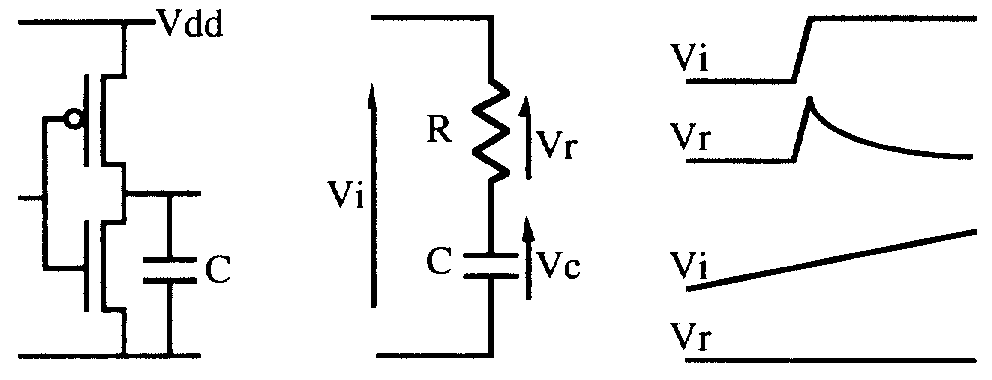
\includegraphics[width=\columnwidth]{../../images/conv_vs_adiabatic.png}
	\caption{Conventional CMOS vs. Adiabatic CMOS in terms of power consumption, shown through the use of the equivalent circuit \cite{DynAdiabatic} }
	\label{fig:convvsadia}
\end{figure}
	\end{column}
\end{columns}

Adiabtic Logic switches much slower, charging up the capacitances with minimal current flow.
There is therefore never a direct short from supply to ground, and heat dissipation is drastically reduced.

In order to achieve the energy saving, adiabatic logic uses a number of stages to set itself up.
Firstly the circuit passes through a \emph{precharge} stage, preloading nodes with a charge.
Then an \emph{evaluation} stage, during which the logical expression is evaluated, and the various nodes either remain charged or discharge as required.
This requirement dictates that adiabatic circuits have a complex clocking circuitry, able to provide two different phases.

\begin{columns}
	\begin{column}{0.49\textwidth}
\begin{figure}
	\centering
	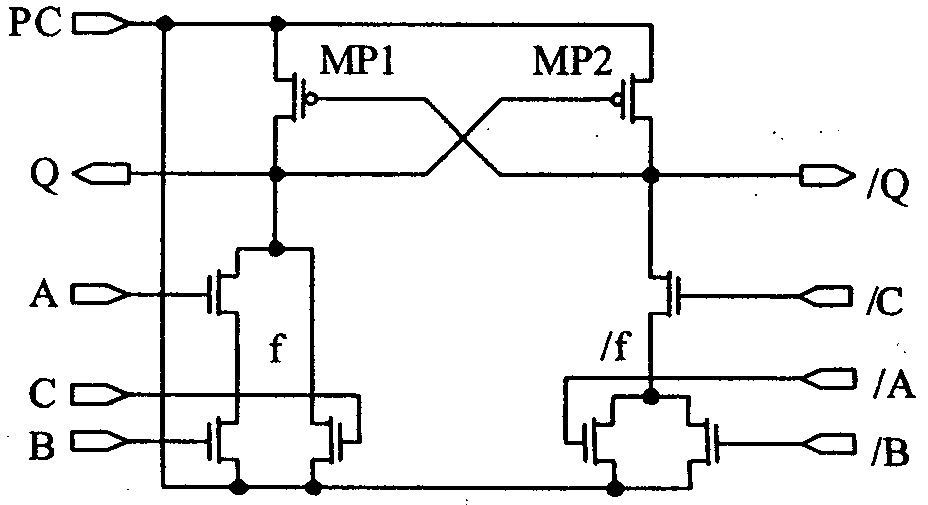
\includegraphics[width=\columnwidth]{../../images/palandor.png}
	\caption{A PAL AND-OR gate ($Q=A.B+C$) showing how to increase the complexity of the circuit \cite{PAL}}
	\label{fig:palandor}
\end{figure}
	\end{column}
	\begin{column}{0.49\textwidth}
		Pass-Transistor Adiabatic Logic (PAL) ia a variation on adiabatic logic requiring only a single clock.
		This clock is sinusoidal, and causes savings of a factor of 10-20.
		Additionally it can provide an inverted output, removing the need for an additional inverter.
	\end{column}
\end{columns}

